% =============================================================================
% SECCIÓN 2.5: LÓGICA DIFUSA Y SISTEMAS DE INFERENCIA MAMDANI
% =============================================================================

\section{Algoritmos}

\subsection{Lógica Difusa y Sistemas de Inferencia Mamdani}
\label{sec:logica_difusa}

La lógica difusa y los sistemas de inferencia Mamdani proporcionan un marco formal para modelar razonamiento humano impreciso mediante variables lingüísticas, conjuntos difusos y reglas del tipo ``SI–ENTONCES'', y se han aplicado extensamente a la clasificación de estados de congestión vehicular en sistemas de transporte inteligente (ITS) \cite{zadeh1965fuzzy,mamdani1975experiment}. Esta sección resume los fundamentos necesarios para entender el diseño del clasificador de congestión utilizado en este trabajo, sin entrar en detalles matemáticos innecesarios.

% -----------------------------------------------------------------------------
\subsubsection{Fundamentos de Lógica Difusa}
% -----------------------------------------------------------------------------

La lógica difusa surge como una generalización de la lógica clásica binaria para tratar conceptos vagos como ``bajo'', ``medio'' o ``alto'', donde la pertenencia de un elemento a una clase no es dicotómica sino gradual \cite{zadeh1965fuzzy}. Zadeh introduce la noción de conjunto difuso mediante una función de membresía que asigna a cada valor numérico un grado de pertenencia entre 0 y 1, permitiendo representar formalmente la idea de ``parcialmente verdadero'' \cite{zadeh1965fuzzy,zadeh1971similarity}. Esta formalización extiende operaciones clásicas como unión, intersección y complemento a un contexto continuo y resulta especialmente útil en dominios donde los límites entre categorías no son nítidos, como en la transición entre tráfico ``fluido'', ``denso'' o ``congestionado''.

En este marco, una variable lingüística es una variable cuyo dominio se describe mediante términos lingüísticos (por ejemplo, la variable ``velocidad'' con valores ``muy baja'', ``baja'', ``media'', ``alta'', ``muy alta''), y cada término se representa como un conjunto difuso sobre el dominio numérico correspondiente \cite{zadeh1971similarity}. Una proposición difusa del tipo ``la velocidad es alta'' se evalúa obteniendo el grado de pertenencia del valor numérico observado al conjunto difuso asociado al término ``alta''. Esta capacidad de trabajar con grados intermedios en lugar de clasificaciones crisp basadas en umbrales fijos es clave para capturar la subjetividad con la que los conductores y los ingenieros perciben la congestión.

% -----------------------------------------------------------------------------
\subsubsection{Funciones de Membresía}
% -----------------------------------------------------------------------------

Las funciones de membresía determinan la forma de los conjuntos difusos e influyen directamente en la suavidad del razonamiento y en la sensibilidad del sistema. En aplicaciones de control e ITS se utilizan habitualmente funciones de tipo triangular, trapezoidal y gaussiana, debido a su simplicidad y a la facilidad de parametrización \cite{ross2010fuzzy}.

En términos prácticos:

\begin{itemize}
    \item Las funciones \textbf{triangulares} se definen por tres parámetros que controlan el inicio, el pico y el final de la región de pertenencia. Ofrecen una transición lineal simple y son muy utilizadas cuando se buscan modelos ligeros computacionalmente.
    \item Las funciones \textbf{trapezoidales} añaden una meseta central donde el grado de pertenencia es máximo, lo que permite representar intervalos de valores considerados claramente pertenecientes a una categoría (por ejemplo, un rango de velocidades que todos los expertos consideran ``medias'').
    \item Las funciones \textbf{gaussianas} proporcionan transiciones suaves e infinitamente diferenciables alrededor de un valor central, resultando útiles cuando se desea un comportamiento más regular o se combinan sistemas difusos con técnicas de optimización continua.
\end{itemize}

En este trabajo se utilizan funciones triangulares y trapezoidales, por su equilibrio entre interpretabilidad, facilidad de ajuste a partir de datos empíricos y bajo costo computacional, siguiendo recomendaciones habituales en control difuso \cite{ross2010fuzzy}. La Figura~\ref{fig:fuzzy_velocidad} ilustra una variable lingüística ``velocidad promedio'' con tres términos (baja, media, alta) definidos mediante este tipo de funciones de membresía.

\begin{figure}[htbp]
\centering
\shorthandoff{>}
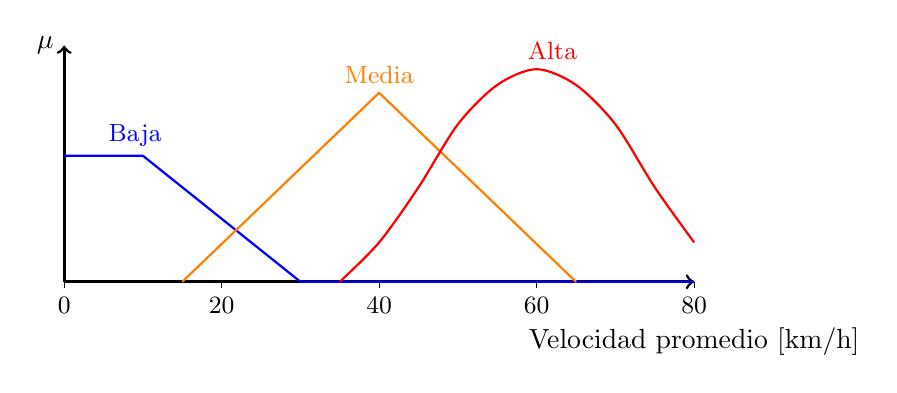
\begin{tikzpicture}[scale=1.0]
    % Ejes
    \draw[->,line width=1pt] (0,0) -- (8,0) node[below,yshift=-0.45cm] {Velocidad promedio [km/h]};
    \draw[->,line width=1pt] (0,0) -- (0,3.0) node[left] {$\mu$};

    % Marcas en eje x
    \foreach \x/\label in {0/0,2/20,4/40,6/60,8/80} {
        \draw (\x,0) -- (\x,-0.08) node[below] {\small \label};
    }

    % Baja: trapezoidal
    \draw[thick,blue]
        (0,1.6) -- (1,1.6) -- (3,0) -- (8,0);
    \node[blue,above] at (0.9,1.6) {\small Baja};

    % Media: triangular
    \draw[thick,orange]
        (1.5,0) -- (4,2.4) -- (6.5,0);
    \node[orange,above] at (4,2.4) {\small Media};

    % Alta: gaussiana aproximada
    \draw[thick,red,smooth] plot coordinates
        {(3.5,0) (4.0,0.5) (4.5,1.2) (5.0,2.0) (5.5,2.5) (6.0,2.7)
         (6.5,2.5) (7.0,2.0) (7.5,1.2) (8.0,0.5)};
    \node[red,above] at (6.2,2.7) {\small Alta};
\end{tikzpicture}
\shorthandon{>}
\caption{Variable lingüística \emph{velocidad promedio} con tres conjuntos difusos (baja, media, alta) modelados mediante funciones de membresía trapezoidal, triangular y aproximadamente gaussiana \cite{ross2010fuzzy}.}
\label{fig:fuzzy_velocidad}
\end{figure}

% -----------------------------------------------------------------------------
\subsubsection{Sistema de Inferencia Mamdani}
% -----------------------------------------------------------------------------

El sistema de inferencia de tipo Mamdani fue introducido por Mamdani y Assilian como un enfoque para implementar controladores basados en reglas lingüísticas expresadas por expertos humanos \cite{mamdani1975experiment}. En este tipo de sistema tanto los antecedentes como los consecuentes de las reglas son conjuntos difusos, y la salida final se obtiene mediante un proceso de defuzzificación que transforma un conjunto difuso agregado en un valor numérico utilizable para control o decisión.

La arquitectura de un sistema Mamdani se organiza típicamente en cuatro etapas \cite{ross2010fuzzy,izquierdo2018mamdani}:

\begin{enumerate}
    \item \textbf{Fuzzificación}: las entradas numéricas (por ejemplo, velocidad promedio, densidad vehicular, flujo) se transforman en grados de pertenencia a los conjuntos difusos definidos para cada variable lingüística. Esto genera un conjunto de etiquetas lingüísticas activadas con diferentes intensidades.
    \item \textbf{Evaluación de reglas}: cada regla del tipo
    \[
      \text{SI velocidad es alta Y densidad es alta ENTONCES congestión es severa}
    \]
    combina los grados de pertenencia de sus antecedentes mediante operadores lógicos difusos (por ejemplo, mínimo o producto para el operador ``Y''), obteniendo un grado de activación para la regla.
    \item \textbf{Agregación}: las salidas difusas de todas las reglas se combinan en un único conjunto difuso de salida, usualmente mediante el operador máximo punto a punto sobre el universo de discurso de la variable de salida.
    \item \textbf{Defuzzificación}: el conjunto difuso agregado se transforma en un valor crisp. El método de defuzzificación más empleado es el centroide (o centro de gravedad), que entrega un valor representativo de la distribución resultante.
\end{enumerate}

La Figura~\ref{fig:mamdani_flujo} resume este flujo de información para el caso específico del problema de congestión vehicular considerado en este trabajo.

\begin{figure}[htbp]
\centering
\shorthandoff{>}
\begin{tikzpicture}[node distance=1.2cm,>=latex]

    \tikzstyle{block} = [rectangle, draw, rounded corners,
                         text width=5cm, align=center,
                         minimum height=0.9cm, font=\small]
    \tikzstyle{line} = [draw,->]

    \node[block] (inputs) {Entradas \emph{crisp}:\\ velocidad promedio, densidad, flujo};
    \node[block, below=of inputs] (fuzz) {Fuzzificaci\'on:\\ c\'alculo de grados de pertenencia};
    \node[block, below=of fuzz] (rules) {Base de reglas Mamdani:\\ combinaci\'on de etiquetas ling\"u\'isticas};
    \node[block, below=of rules] (agg) {Agregaci\'on:\\ unificaci\'on de salidas difusas};
    \node[block, below=of agg] (defuzz) {Defuzzificaci\'on:\\ c\'alculo de nivel de congesti\'on \emph{crisp}};
    \node[block, below=of defuzz] (output) {Salida:\\ nivel de congesti\'on o se\~nal de control};

    \path[line] (inputs) -- (fuzz);
    \path[line] (fuzz) -- (rules);
    \path[line] (rules) -- (agg);
    \path[line] (agg) -- (defuzz);
    \path[line] (defuzz) -- (output);

\end{tikzpicture}
\shorthandon{>}
\caption{Etapas principales de un sistema de inferencia difusa tipo Mamdani aplicado a congestión vehicular \cite{mamdani1975experiment,izquierdo2018mamdani}.}
\label{fig:mamdani_flujo}
\end{figure}

% -----------------------------------------------------------------------------
\subsubsection{Aplicación en Clasificación de Congestión Vehicular}
% -----------------------------------------------------------------------------

En sistemas de transporte inteligente, la lógica difusa se utiliza ampliamente para modelar la percepción humana de la congestión y para construir clasificadores que estimen el estado del tráfico a partir de variables macroscópicas como flujo, velocidad y densidad \cite{erdinc2023application,musriroh2020application}. La representación gradual de conceptos como ``flujo alto'' o ``velocidad baja'' permite evitar umbrales rígidos, lo que hace que estos modelos sean menos sensibles al ruido de las mediciones y más cercanos a la forma en que los operadores interpretan la situación de tráfico.

Un esquema típico de clasificación difusa de congestión vehicular con sistema Mamdani incluye:

\begin{itemize}
    \item \textbf{Selección de variables de entrada}: se utilizan variables como flujo (vehículos/hora), velocidad media (km/h) y densidad (vehículos/km); en algunos casos se añaden métricas como ocupación o tiempo de viaje para capturar mejor la variabilidad del tráfico \cite{erdinc2023application}.
    \item \textbf{Definición de variables lingüísticas}: cada variable se discretiza en términos como ``bajo'', ``medio'', ``alto'' o ``muy alto'', representados mediante funciones de membresía triangulares o trapezoidales ajustadas a partir de datos históricos o de la experiencia de expertos \cite{musriroh2020application}.
    \item \textbf{Base de reglas}: se construye un conjunto de reglas del tipo ``SI flujo es alto Y velocidad es baja Y densidad es alta ENTONCES congestión es severa'', que codifican el conocimiento experto o patrones empíricos.
    \item \textbf{Inferencia y clasificación}: el sistema Mamdani procesa en tiempo (casi) real las mediciones de los sensores y devuelve un nivel de congestión que se defuzzifica a categorías discretas como \{libre, estable, inestable, congestionado\} \cite{erdinc2023application,musriroh2020application}.
\end{itemize}

Diversos estudios reportan que los clasificadores difusos basados en Mamdani son robustos ante datos incompletos o ruidosos y capturan de manera más fiel la percepción de los usuarios respecto a soluciones crisp basadas en umbrales fijos \cite{erdinc2023application,musriroh2020application,esmaeili2025optimization}. Por ejemplo, Erdinç propone un identificador difuso de estado de tráfico que utiliza flujo, velocidad y densidad como entradas y demuestra que el modelo reproduce correctamente las transiciones entre flujo libre y condiciones hipercríticas en escenarios simulados \cite{erdinc2023application}. Otros trabajos aplican lógica difusa Mamdani al control de semáforos y a la gestión dinámica de carriles, mostrando reducciones significativas en tiempos de viaje y número de paradas frente a esquemas de control fijo \cite{musriroh2020application,esmaeili2025optimization}.

En el contexto de este trabajo, estos resultados justifican la elección de un sistema de inferencia Mamdani para clasificar el grado de congestión urbano a partir de variables macroscópicas, proporcionando una salida interpretable (leve, moderada, severa) que puede integrarse de forma natural con los módulos de optimización y control semafórico desarrollados en capítulos posteriores.